% Created 2022-11-29 Tue 11:06
% Intended LaTeX compiler: pdflatex
\documentclass[11pt,a4paper]{article}
    \usepackage[utf8]{inputenc}
    \usepackage[T1]{fontenc}
    \usepackage{fixltx2e}
    \usepackage{graphicx}
    \usepackage{longtable}
    \usepackage{float}
    \usepackage{wrapfig}
    \usepackage{rotating}
    \usepackage[normalem]{ulem}
    \usepackage{amsmath}
    \usepackage{textcomp}
    \usepackage{marvosym}
    \usepackage{wasysym}
    \usepackage{amssymb}
    \usepackage{hyperref}
    \usepackage{mathpazo}
    \usepackage{color}
    \usepackage{enumerate}
    \definecolor{bg}{rgb}{0.95,0.95,0.95}
    \tolerance=1000
                    \usepackage{listings}
\usepackage{xcolor}
\lstset{language=Python,backgroundcolor=\color{black!5}, basicstyle=\footnotesize\ttfamily, columns=fullflexible, breaklines, frame= tb}

    \linespread{1.1}
    \hypersetup{pdfborder=0 0 0}
\author{Ved Patel 67 Vijay Panchal 68}
\date{\today}
\title{Timebomb of approximation in physics}
\hypersetup{
 pdfauthor={Ved Patel 67 Vijay Panchal 68},
 pdftitle={Timebomb of approximation in physics},
 pdfkeywords={},
 pdfsubject={},
 pdfcreator={Emacs 28.1 (Org mode 9.5.2)}, 
 pdflang={English}}
\begin{document}

\maketitle
\tableofcontents

\pagebreak
\section{Introduction}
\label{sec:org2832ecd}

Approximation method is yet most essential topic in physics. Also, approximation is yet essential trick for physicists. Physicists love to do approximations, like in functional expansion for getting polynomials for their ease or may be specialized idealization in particular topic. Approximation help them to \textbf{seeing through physics} instead of going in to maze of exactness in formidable  mathematics. Getting interpretation or i say knowing system is sometime more important then going for regorious mathematics. For example, famous equation of fluid dynamics \textbf{Navier-Stoke equation} can be imposible to solve but as physicist they know what it is.

Be aware, that approximation is just approximation. We should remember everytime we do that. Sometime we forgot actual system which is far from ideal. We should know that we are on mission to know nature not just building new theories.

Let's dive into one example, that showes implication of approximations. In classical mechanics, we have some major theories, one is of oscillatory motions. In Oscillation theory we studied \textbf{Simple Harmonic Oscillation}, but as we are going to see that simple harmonic oscillation is not exactly that simple without approximation. We had actually changed whole system unknowingly, but beauty of physics is that it is still help to understand concept and motion of it. 

\section{Example of Approximation}
\label{sec:org994e3a4}

Approximation is used in almost every branch of physics, not just physics but every field of sciences. We are going to give profound example of understanding advantages and disadvantages of approximation.

\subsection{Defining a problem}
\label{sec:orgac3f1ab}

We learned simple pendulum from very starting of physics course. But what if i say that simple pendulum is not actually simple in sense that approximation hide most of things away from our eyes to see.

Let's take one pendulum,by taking length \(l = 1 m\) string (assuming non deforming) attaching to bob of mass \(m = 0.1 kg\). String attached to rigid wall as shown in figure. Then we give it a initial deviation. We have accelaration of \(g=9.8\) downward.

\begin{figure}[htbp]
\centering
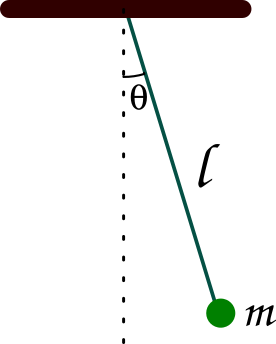
\includegraphics[width=0.3 \textwidth]{./figure1.png}
\caption{\label{fig:orgab0b11b}pendulum with string lenth \(l\) and mass \(m\)}
\end{figure}

For understanding consequences of approximation, we took simulations by solving both equation of motion (approximated and exact). For getting equations of motion we used \textbf{Newtonian formulation} which is quite easy to work with in this type of problems, since we are working with \textbf{non conservative} system.


\subsection{Pendulum motion in presence of damping force}
\label{sec:org9f9e7f6}

In real situations we have non-conservative forces affecting on system. In our system we have air resistance acting on bab. This drag force will always be proportional to it's physical shape and size. Since, we can't tell exactly drag force mathematically, We have \textbf{two often used approximations}. Firstly, there is stockes's law which is linearly proportional to the velocity. Then we have Newton's drag law which is quadratically proportional to the velocity. \textbf{\textbf{[1]}}   



First of all, we took horizontal and vertical forces.
\begin{equation}
\label{eq:orga01b24f}
   F_{damping}cos(\theta)-Tsin(\theta)=ma_{x}
\end{equation}
\begin{equation}
\label{eq:orged11d8f}
   F_{damping}sin(\theta)+Tcos(\theta)-mg=ma_{y}
\end{equation}

Adding equation \ref{eq:orga01b24f} and equation \ref{eq:orged11d8f} with multiplication by \(cos(\theta)\) and \(sin(\theta)\) respectively.

\begin{equation*}
\label{eq:org1654464}
F_{damping}sin^{2}(\theta)+F_{damping}cos^{2}(\theta)-mgsin(\theta)=ma_{x}cos(\theta)+ma_{y}sin(\theta)
\end{equation*}

\begin{equation*}
\label{eq:org877166e}
F_{damping}-mgsin(\theta)=m(asin^{2}(\theta)+acos^{2}(\theta))
\end{equation*}

\begin{equation}
\label{eq:orgbd84f0f}
F_{damping}-mgsin(\theta)=ma
\end{equation}

From,
\begin{equation*}
\label{eq:org20d75d8}
a = (\ddot{r}-r\dot{\theta}^{2})\hat{r} + (r \ddot{\theta}+2\dot{r}\dot{\theta})\hat{\theta}
\end{equation*}

Where,  \(r=l\) and since \(\dot{l}=0\), \(a=l\ddot{\theta}\). So, equation \ref{eq:orgbd84f0f} becomes,

\begin{equation*}
\label{eq:org9f84f10}
F_{damping}-mgsin(\theta)=ml\ddot{\theta}
\end{equation*}

We are taking damping force to velocity proportional. So, \(F_{damping}=-bl\dot{\theta}\) ( since, \(\dot{l}=0\)). Here, we are assuming that damping is linear. 

\begin{equation*}
\label{eq:org254e8b7}
-bl\dot{\theta}-mgsin(\theta)=ml\ddot{\theta}
\end{equation*}


Rearranging this equation will give our equation of motion,

\begin{equation}
\label{eq:org00bdaf7}
\ddot{\theta}+\frac{b}{m}\dot{\theta}+\frac{g}{l}sin(\theta)=0
\end{equation}

This is \textbf{exact equation of motion}. Which is \textbf{second order non linear equation}. Finding it's exact solution is massive task. We will use numerical methods to find it's solution. This equation has much more to say than looks. Will learn about this in later.

\subsection{Approximation of equation of motion : Linear differential equation}
\label{sec:org0518d21}

Solving \ref{eq:org00bdaf7} is very hard tasks. So, we as physics majors try to make this as friendly as possible. In class, we approximated this as \(\theta \to 0\) as \(sin(\theta) \to \theta\). Consequently, this equation becomes very easy to solve. This becomes,

\begin{equation}
\label{eq:org2a3279e}
\ddot{\theta}+\frac{b}{m}\dot{\theta}+\frac{g}{l}\theta=0
\end{equation}

\begin{equation}
\label{eq:org38f388f}
\ddot{\theta}+\Gamma\dot{\theta}+w_{0}^{2}\theta=0
\end{equation}

Where we took \(\Gamma = \frac{b}{m}\) and \(w_{0}^{2}\).

We can solve this linear equation \ref{eq:org38f388f} by usual methods of linear differential equation. Simply taking \(\theta=e^{\lambda t}\), which gives polynomials of second order.

\begin{equation}
\label{eq:org6d5f5aa}
\lambda^{2}+\Gamma\lambda+w_{0}^{2}=0
\end{equation}

We can find roots of this quadratic equation.

\begin{equation}
\label{eq:org4a1c80c}
\lambda = \frac{-\Gamma}{2} \pm \frac{\sqrt{\Gamma^{2}-4w_{0}^{2}}}{2}
\end{equation}

\begin{equation}
\label{eq:org29a5e8b}
\lambda = \frac{-\Gamma}{2} \pm \sqrt{\frac{\Gamma}{2}^{2}-w_{0}^{2}}
\end{equation}

Here we getting three type of roots,

\begin{enumerate}
\item Roots where \(\frac{\Gamma}{2}=w\). this is \textbf{critical damping condition}, where we getting \(\lambda=\frac{-\Gamma}{2}\). Putting \(\lambda\) into our solutions, \(\theta = e^{\frac{-\Gamma}{2}t}\). Which suggest this will only decay with time and never overshoots from equilibrium position. Which is desired in certain condition but not for us.

\item Roots where \(\frac{\Gamma}{2}>w\). this is \textbf{overdamping condition}, where we getting \(\lambda=\frac{-\Gamma}{2}\pm\sqrt{\frac{\Gamma}{2}^{2}-w_{0}^{2}}\). So from here we get \(\theta = e^{\frac{-\Gamma}{2}t}e^{\pm\sqrt{\frac{\Gamma}{2}^{2}-w_{0}^{2}}t}\). This also have exponential term in it which will only decay with time and never overshoots from equilibrium position.

\item Roots where \(\frac{\Gamma}{2}<w\). this is \textbf{underdamping condition}, here  \(\lambda=\frac{-\Gamma}{2}\pm i\sqrt{w_{0}^{2}-\frac{\Gamma}{2}^{2}}\). \(\theta = e^{\frac{-\Gamma}{2}t}e^{\pm i \sqrt{w_{0}^{2}-\frac{\Gamma}{2}^{2}}t}\). This has complex term, which implicitly suggest that it'll overshoot and oscillate. This our topic of interest for this project.
\end{enumerate}


Without forgetting our initial system we came to we took third case as our solution.

\begin{fleqn}
\therefore \qquad \qquad \qquad \qquad \theta = e^{\frac{-\Gamma}{2}t}e^{\pm i \sqrt{w_{0}^{2}-\frac{\Gamma}{2}^{2}}t}
\\
\label{orgf6f592a}
\end{fleqn}

Taking \(w^{2} = w_{0}^{2}-\frac{\Gamma}{2}^{2}\). And writing our solution in linear combination from above equation,

\begin{equation}
\label{eq:org3601395}
\theta = e^{\frac{-\Gamma}{2}t}(C_{1}e^{iwt}+C_{2}e^{-iwt})
\end{equation}

Taking real part of equation \ref{eq:org3601395}. Since it'll represent real motion of system. At last we get equation like this,

\begin{equation}
\label{eq:org41e7a74}
\theta = e^{\frac{-\Gamma}{2}t}A cos(wt-\delta)
\end{equation}

Where, \(A\) and \(\delta\) can be find from initial conditions and \(w = \sqrt{w_{0}^{2}-\frac{\Gamma}{2}^{2}}\).



\subsection{Understanding with little simulations}
\label{sec:org4c19526}

For understaning what is we want to tell. Basically we made simulation of both the equation of motion side by side. This simulation tales that motion of both solution will be very near onto small position where \(\theta\) is quite small, but not from other. We also, try to compare with physical model \textbf{give nice view}.

Firstly exact equation of motion is nonlinear differential equation. We can't get exact solution of it. So, we just use numerical methods. We use \textbf{fourth order Runge-Kutta method}. Basically, we elaborated whole method in short down here. 

\subsubsection{Understand Runge-Kutta method}
\label{sec:orgc0cb7f2}

In our this simulation we made use of Range Kutta fourth order method as numerical method for solving non-linear differential equation and linear differential equation with it. So, it is good idea to understand what is Range-Kutta fourth order method and how can we implement to solve present differential equations.

Runge Kutta Method is not predictor-corrector method like other numerical method (namely, modified Euler method, Adams-Bashmoth-Moulton method) for solving differential equation. It uses four different new variables and then simply addition and multiplication predict our initial value problem with good accuracy.






\subsubsection{Animations}
\label{sec:org3c26531}

Now, come animation part. Which we basically used \textbf{pygame} in \textbf{python}. We first get array of both solutions with interval of \(\frac{1}{60} second\) and give this data in position function in my \emph{main.py} file which just use convert each to the Cartesian coordinates from initial Polar coordinate. This is because \emph{pygame} screen rectangular coordinates with units in pixel of screen.

Following data, we used as constant which i defined in \emph{constant.py} file, as per close inspection you can see that we used C.G.S. units because of better visual on computer screen. Remember, we made this code for reconstruct purpose only.

My \emph{constant.py} file

\begin{lstlisting}language=Python]
  from math import sqrt

  # defining constants in C.G.S.


  width,height = 1360,720         # pygame window size in pixel units
  origin_x,origin_y = width/2,height/8 # setting up the origin O
  b = 100                              # damping coefficient
  m = 100                              # 100 grams of mass
  l = 100                              # 100 cm length
  g = 980                              # gravitation accelaraiotion in cgs

  gamma = b/m

  w0 = sqrt(g/l)                  # natural frequncy of SHM
  theta_initial = 3.141591/4      # initial theta in radian
  radius = 10                     # radius of ball in pixel
  fps = 60                        # frame per second
\end{lstlisting}

This is my \emph{main.py} file, in which i defined all functions for calculations. In which, i have Runge-Kutta method defined and solution and also phase planes defined.

\begin{lstlisting}[language=Python]
  from constants import *
  from numpy import sin, sqrt, zeros

  def f2nonlinear(theta,phi):     # we defined second auxillary equation from nonlinear term.
  return -((gamma/m)*phi*phi)-(w0*sin(theta))

  def f2linear(theta,phi):        # we defined second auxillary equation from linear term.
  return -((gamma/m)*phi*phi)-(w0*theta)

  # range-kutta method defined
  def RK4(t,theta,phi,h,K): 
  h = h/8
  for i in range(8):
  k1 = h*phi
  l1 = h*K(theta,phi)
  k2 = h*(phi+(l1*0.5))
  l2 = h*(K(theta+(k1*0.5),phi+(l1*0.5)))
  k3 = h*(phi+(l2*0.5))
  l3 = h*(K(theta+(k2*0.5),phi+(l2*0.5)))
  k4 = h*(phi+l3)
  l4 = h*(K(theta+k3,phi+l3))
  k_ = (1/6)*(k1+k4+2*(k2+k3))
  l_ = (1/6)*(l1+l4+2*(l2+l3))
  t+=h
  theta+=k_
  phi+=l_
  return  t,theta,phi

  # Solutions of linear term ---- gives array of length (Total_time*fps)
  def linear(theta_initial,Total_time,fps):
  linear_solutions = zeros([Total_time*fps])
  linear_solutions[0] = theta_initial
  phi = zeros([Total_time*fps])
  phi[0],t,time = 0,0,0
  while t-1<Total_time*fps:
  time, linear_solutions[t+1], phi[t+1] = RK4(time,linear_solutions[t],phi[t],1/fps,f2linear)
  t+=1
  return linear_solutions

  # Solutions of nonlinear term ---- gives array of length (Total_time*fps)
  def nonlinear(theta_initial,Total_time,fps):
  nonlinear_solutions = zeros([Total_time*fps])
  nonlinear_solutions[0] = theta_initial
  phi = zeros([Total_time*fps])
  phi[0],t,time = 0,0,0
  while t-1<Total_time*fps:
  time, nonlinear_solutions[t+1], phi[t+1] = RK4(time,nonlinear_solutions[t],phi[t],1/fps,f2nonlinear)
  t+=1
  return nonlinear_solutions


  # ------------(for graphs)----------
  # this describes frequncy of nonlinear term.
  def w_nonliner(theta_initial):
  T = (sqrt(l/g))*(1+(0.24*(sin(0.5*theta_initial))**2)+((9/24)*(sin(theta_initial*0.5))**4))
  return 1/T

  # phase plane definations
  def linear_phase_plane(theta,phi):
  f1 = phi
  f2 = -((gamma/m)*phi*phi)-(w0*sin(theta))
  return f1,f2

  def nonlinear_phase_plane(theta,phi):
  f1 = phi
  f2 = -((gamma/m)*phi*phi)-(w0*sin(theta))
  return f1,f2

  # ----------------------------------

\end{lstlisting}

\section{What is meaning of all this ?}
\label{sec:org5d33c53}
\section{Appendix}
\label{sec:org0693602}

This is my simulation fi

\section{References}
\label{sec:org2a1b454}

[1] Lubarda, Marko V., and Vlado A. Lubarda. "An analysis of pendulum motion in the presence of quadratic and linear drag." Eur. J. Phys 42.055014 (2021): 055014.
\end{document}